%!TeX root=20_Hauptteil.tex

\chapter{Stand der Technik}

Dieses Kapitel gibt einen Überblick über den aktuellen Stand der Technik im Bereich 
der \gls{gnss}-freien Lokalisierung von \gls{uav} und ordnet die in dieser Arbeit 
gewählten Methoden in den wissenschaftlichen Kontext ein.
Zunächst werden bestehende Lokalisierungsansätze ohne \gls{gnss} vorgestellt und hinsichtlich ihrer Eignung für Innenraumanwendungen bewertet.
Anschließend werden verschiedene Fiducial-Marker-Systeme verglichen und deren Eigenschaften im Hinblick auf die Anforderungen dieser Arbeit diskutiert.
Abschließend wird auf die simultane Lokalisierung und Kartierung eingegangen, die die Grundlage für die in dieser Arbeit verwendete Kartierungsmethodik bildet.

\section{GNSS-freie Lokalisierung von UAVs}
Die Navigation ohne \gls{gnss} stellt in der Luftfahrt eine erhebliche Herausforderung dar, da \gls{gnss} als primäre Quelle absoluter Positionsinformationen dient.
In dessen Abwesenheit muss die Position aus der Integration fehlerbehafteter Inertialmessungen 
geschätzt werden, was, wie in Abschnitt \ref{sec:Sensorsysteme} beschrieben, zu einem zeitlich anwachsenden Positionsfehler führt.
Daher ist es notwendig, diesen Fehler durch absolute oder relative Lokalisierungsmethoden auszugleichen.\cite{Jarraya2025}


\subsection{Absolute Lokalisierung}
Absolute Lokalisierungsverfahren spielen eine wichtige Rolle, wenn die genaue Position eines \gls{uav} bezogen auf einen globalen Referenzrahmen bekannt sein muss.\cite{Jarraya2025}
Die gängigste Methode zur Umsetzung einer absoluten Lokalisierung ist ein satellitengestütztes System wie \gls{gps} oder Galileo.
Da in der für diese Arbeit relevanten Flugumgebung kein ausreichender Satellitenempfang herrscht, finden diese Systeme keine Anwendung.
Eine weitere Möglichkeit der absoluten Lokalisierung bieten Template- und Feature-basierte Verfahren sowie Semantic Mapping.

Bei Template- beziehungsweise Feature-basierten Verfahren werden Aufnahmen des \gls{uav} mit bekannten Referenzbildern oder gespeicherten Merkmalen verglichen.
Diese Systeme berücksichtigen ausschließlich visuelle Merkmale, ohne semantische Beziehungen einzubeziehen.\cite{Jarraya2025}
Ein verwandtes Konzept stellen Fiducial-Marker dar, bei denen anstelle natürlicher Bildmerkmale künstlich erzeugte, eindeutig kodierte Muster als Referenz dienen.
Durch ihre definierte Geometrie und Kodierung ermöglichen sie eine präzisere und robustere Posenschätzung als natürliche Bildmerkmale, weshalb sie in dieser Arbeit 
als Grundlage der Lokalisierung eingesetzt werden.
Im Sinne einer globalen absoluten Lokalisierung im Weltkoordinatensystem sind Template- und Feature-basierte Verfahren für Innenraumanwendungen jedoch wenig geeignet, 
da geeignete Referenzdaten schwer zu erfassen sind.\cite{Jarraya2025}

Semantic Mapping verfolgt einen ähnlichen Ansatz: Auch hier werden zunächst Referenzdaten 
erstellt, die anschließend mit aktuell erfassten Daten abgeglichen werden.
Der Unterschied liegt darin, dass nicht nur visuelle Merkmale, sondern auch semantische 
Beziehungen berücksichtigt werden, so wird beispielsweise ein Tisch als Tisch und eine 
Treppe als Treppe interpretiert.\cite{Jarraya2025}
Dieses Verfahren findet in der vorliegenden Arbeit keine Anwendung, da die Erkennungsleistung stark von der Stabilität der jeweiligen Umgebung abhängig ist.

Da die einzige praktikabel umsetzbare Methode der absoluten Lokalisierung ein 
satellitengestütztes System darstellt, welches wie bereits erwähnt in der vorliegenden Umgebung nicht verfügbar ist, wird in dieser Arbeit auf absolute Lokalisierungsverfahren verzichtet 
und ausschließlich relative Lokalisierungsmethoden betrachtet.
Die grundlegende Methodik der zuvor vorgestellten Verfahren findet dabei ebenfalls Anwendung, jedoch ohne Bezug zu einem globalen Referenzrahmen.

\subsection{Relative Lokalisierung}
\label{sec:relative_lokalisierung}
Die relative Lokalisierung zielt darauf ab, die Position und Orientierung eines \gls{uav} innerhalb eines lokalen Koordinatensystems zu bestimmen.
Die Position wird dabei bezogen auf einen definierten Referenzpunkt ermittelt.
Im Folgenden werden die gängigsten Methoden vorgestellt und hinsichtlich ihrer Eignung für die vorliegende Innenraumanwendung bewertet.

\subsubsection{Dead Reckoning Localization}
Bei der \gls{drl} handelt es sich um ein Verfahren, bei dem die aktuelle Position eines 
Objekts ausgehend von einem letzten bekannten Startpunkt kontinuierlich berechnet 
wird.\cite{9982087}
Die Berechnung erfolgt auf Basis der bereitgestellten \gls{imu}-Daten durch Integration 
dieser.
Wie in Abschnitt \ref{sec:sensorik} bereits beschrieben, wirken auf die Sensoren erhebliche 
Fehler, sodass die direkte Integration der rohen \gls{imu}-Messdaten zu großen 
Translationsfehlern führt.
Aus diesem Grund ist eine Filterung der Eingangsdaten notwendig.
Am weitesten verbreitet sind hierbei verschiedene Abwandlungen des Kalman-Filters.

Experimentelle Untersuchungen mit dem \gls{px4}-Autopiloten und einem handelsüblichen 
Pixhawk-Flugregler zeigen, dass der \gls{ekf2} bereits nach 7 Sekunden eine 
Geschwindigkeitsabweichung von $\sigma_{\text{vel}} \approx 0{,}024$~m/s aufweist, was zu 
einem zunehmenden Positionsfehler im Dezimeterbereich führt.\cite{9172736}
Verschiedene Arbeiten zeigen, dass sich der Drift vor allem durch Nutzung verbesserter 
Algorithmen wie dem \gls{iekf} minimieren, jedoch nicht vollständig vermeiden lässt.
\cite{9982087}\cite{9172736}\cite{Ko2018}
Da im verwendeten Flugcontroller, wie in Kapitel \ref{sec:Pixhawk_6X} beschrieben, der 
\gls{ekf} implementiert ist, wird nicht weiter auf andere Abwandlungen des Algorithmus 
eingegangen.

Grundsätzlich ist \gls{drl} für den Innenraum nur zeitlich begrenzt geeignet und als 
primäre Positionsquelle nicht ausreichend.
Im Normalfall wird \gls{drl} daher als Fallback-Strategie genutzt, wenn die primäre 
Positionsquelle nicht verfügbar ist.\cite{9172736}
In dieser Arbeit wird der Flugcontroller entsprechend konfiguriert.


\subsubsection{Visuelle Odometrie und optischer Fluss}
Visuelle Odometrie sowie optischer Fluss sind grundlegende Verfahren zur Lokalisierung eines \gls{uav}.
Die \gls{vo} schätzt die Bewegung einer Kamera anhand sequenzieller Bilddaten, ohne eine Karte der Umgebung zu erstellen.
Dabei werden markante Bildpunkte, auch Landmarken genannt, zwischen aufeinanderfolgenden Frames verfolgt und aus deren Verschiebung auf die Kamerabewegung geschlossen.\cite{Jarraya2025}

Darüber hinaus existieren \gls{vio}-Ansätze, die die Robustheit der \gls{vo} durch Einbeziehen von \gls{imu}-Informationen verbessern.\cite{9836067}
Die visuellen Daten können dabei den Drift der \gls{imu} reduzieren, während die \gls{imu}-Daten den metrischen Maßstab sowie Roll- und Nickwinkel aus den visuellen 
Daten wiederherstellen können.\cite{9836067}
Es gibt sowohl mono- als auch stereokamerabasierte Ansätze, wobei Stereokameras aufgrund der direkten Tiefenschätzung eine höhere Genauigkeit erzielen.\cite{9836067}
Die Fusion von \gls{imu} und \gls{vo} zu \gls{vio} erfolgt typischerweise über einen \gls{ekf}.\cite{9836067}

Da \gls{vo} und \gls{vio} keinen absoluten Positionsbezug besitzen, akkumulieren diese Verfahren über die Zeit einen Drift und sind damit nur bedingt für eine langfristig stabile Innenraumlokalisierung geeignet.\cite{Jarraya2025}
Zudem ist die Leistung kamerabasierter Verfahren stark von den Lichtverhältnissen der Umgebung abhängig.\cite{9836067}
Weiterhin visuelle Odometrie setzt strukturierte Umgebungen voraus, welche in der Versuchsumgebung nicht ohne weiteres gegeben sind. 

Der optische Fluss stellt ein verwandtes Verfahren dar, das im Gegensatz zur \gls{vo} 
lediglich zweidimensionale Geschwindigkeitsinformationen liefert.\cite{Jarraya2025}
Aus diesem Grund ist der optische Flow nicht zur Positionserkennung einer \gls{uav} geeignet.


\subsection{Simultane Lokalisierung und Kartierung}
\gls{slam} beschreibt eine Problemstellung an der Schnittstelle von Computer Vision und Robotik.
Dabei geht es um die selbstständige Erstellung einer Karte einer unbekannten Umgebung bei gleichzeitiger Bestimmung der eigenen Position 
innerhalb dieser Umgebung.\cite{10169695}
Der Begriff simultan beschreibt genau diesen Zusammenhang: 
Kartierung und Positionsbestimmung müssen parallel erfolgen, da jede Aufgabe die andere voraussetzt.\cite{10169695}
Die Lösung dieses Problems erfolgt üblicherweise durch filterbasierte Methoden, wie den \gls{ekf}, oder durch optimierungsbasierte Methoden, die im Folgenden 
näher beschrieben werden.\cite{10169695}

Filterbasierte \gls{slam} Algorithmen verarbeiten Messungen sequenziell und lassen keine Korrektur von vergangenen Messungen zu.
Insbesondere fehlt filterbasierten Methoden die Fähigkeit zur globalen Kartenkorrektur durch Loop Closure, 
was zu einer geringeren Kartierungsgenauigkeit im Vergleich zu optimierungsbasierten Methoden führt.
In der Lokalisierung sind filterbasierte Methoden aufgrund ihrer geringeren Rechenkomplexität jedoch schneller.\cite{10169695}
Der aktuelle Standard bei \gls{slam}-Algorithmen sind optimierungsbasierte Methoden.
 

\subsubsection{Phasen optimierungsbasierter SLAM Methoden}
\label{sec:phasen_slam}
Der allgemeine optimierungsbasierte \gls{slam}-Prozess lässt sich in folgende Phasen unterteilen:

\textbf{Feature Extraction} bezeichnet die Extraktion markanter Merkmale 
aus den Sensordaten, die als Grundlage für die spätere Zuordnung dienen.\cite{10169695}

\textbf{Feature Matching} beschreibt den Abgleich extrahierter Merkmale zwischen 
aufeinanderfolgenden Frames, um die Bewegung des Systems zu schätzen.\cite{10169695}
Beispiele dieser Methoden werden in Abschnitt \ref{sec:relative_lokalisierung} beschrieben.

\textbf{Map Initialization} bezeichnet die Initialisierung der Karte zu Beginn des \gls{slam}-Prozesses.
Dabei werden zunächst markante Bildmerkmale aus den ersten Frames extrahiert und 
einander zugeordnet, um die initiale Struktur der Umgebung zu schätzen.
Aus diesen Zuordnungen werden erste Kartenpunkte sowie deren räumliche Positionen im dreidimensionalen Raum bestimmt.
Die Map Initialization bildet die Grundlage, auf der alle weiteren Kartenpunkte und Posenschätzungen aufgebaut werden. \cite{vslam_core_modules_2024}

\textbf{Loop Closure} bezeichnet die Erkennung bereits besuchter Orte.
Wird ein solcher Ort erkannt, wird die akkumuliert Abweichung anhand gespeicherter Merkmale berechnet und als zusätzlicher Constraint den Faktorgraphen eingetragen. 
Die anschließende globale Optimierung verbessert die Konsistenz der gesamten Karte erheblich. \cite{10169695} 
Der schematische Ablauf von Loop Closure ist in Abbildung~\ref{fig:loop_closure} dargestellt.
Die Funktion des Faktorgraph wird in Abschschnitt \ref{sec:Faktorgraph} näher beschrieben.
\begin{figure}[htbp]
    \centering
    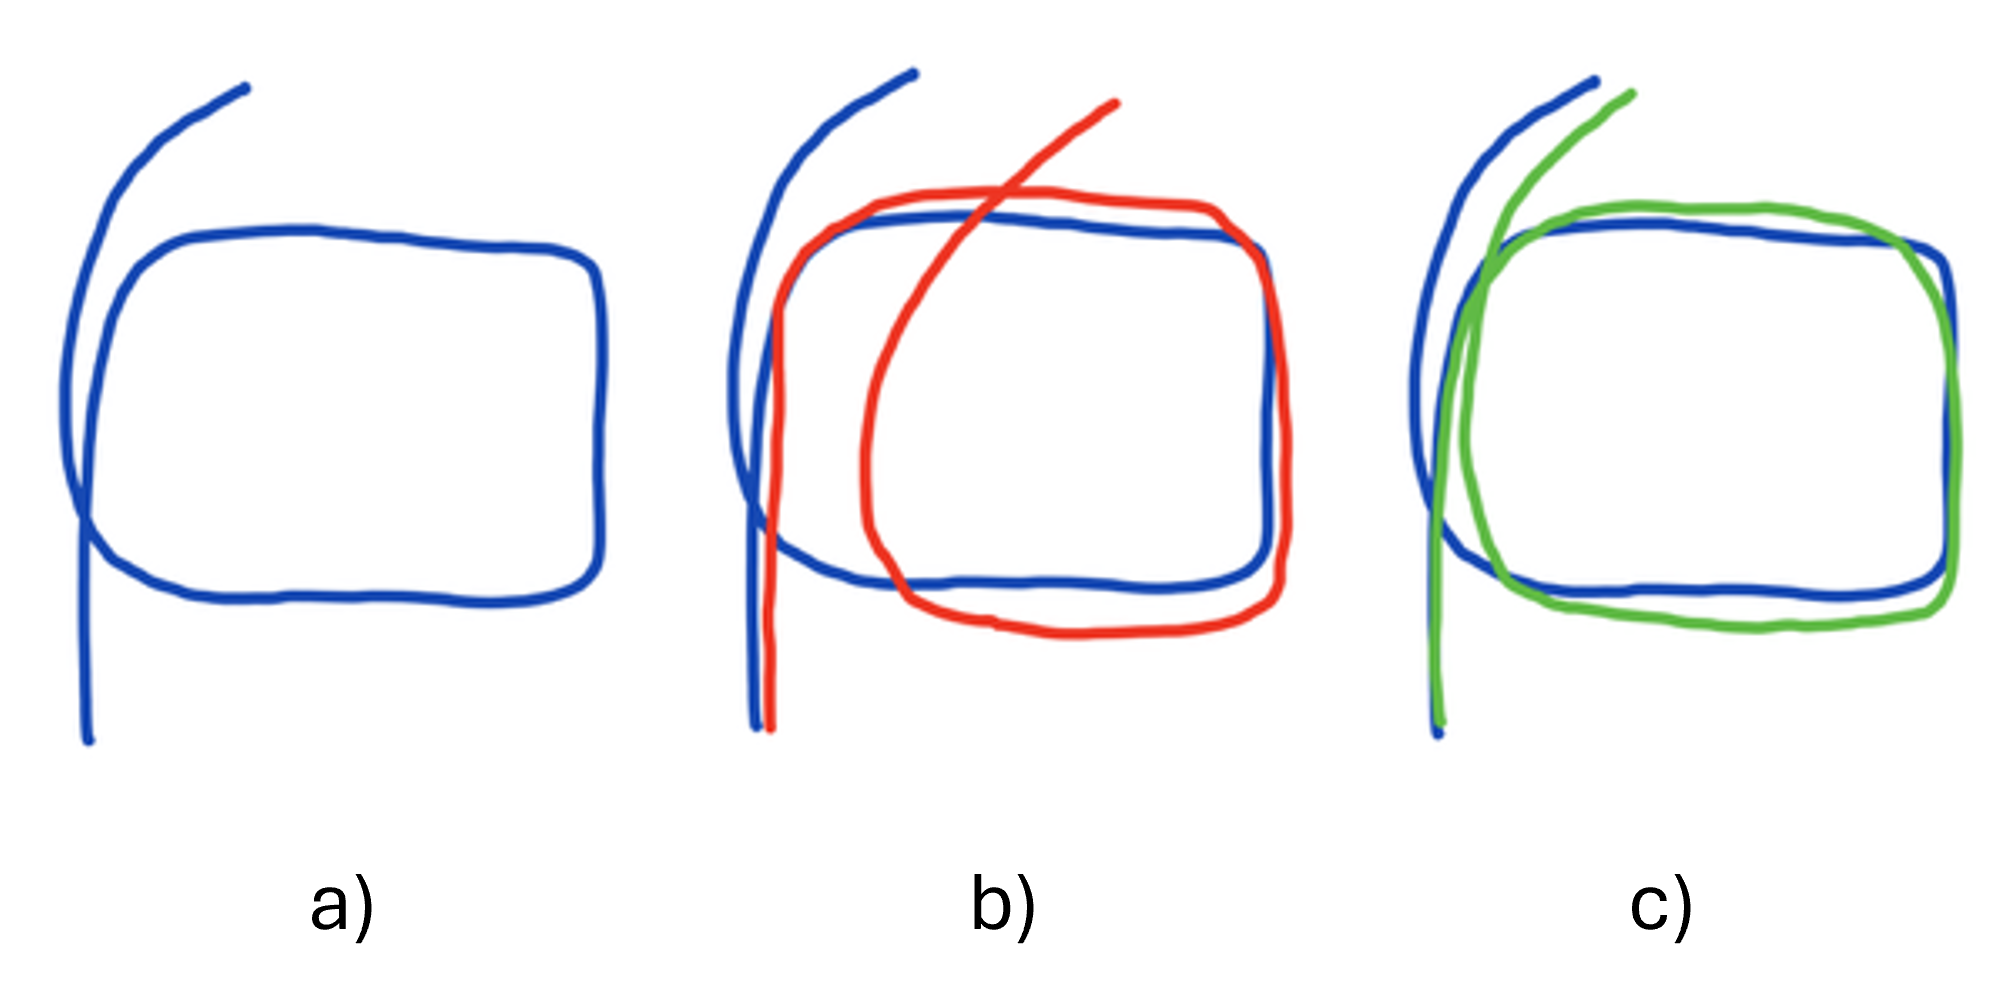
\includegraphics[width=1.0\textwidth]{Bilder/Loop_Closure.png}
    \caption{Veranschaulichung des Loop-Closure-Effekts: 
    (a) Reale Trajektorie ohne akkumulierten Fehler. 
    (b) Geschätzte Trajektorie mit akkumuliertem Drift ohne Loop Closure. 
    (c) Korrigierte Trajektorie nach Anwendung von Loop Closure mit 
    reduziertem akkumuliertem Drift. vgl. \cite{gong_loop_closure}}
    \label{fig:loop_closure}
\end{figure}
\FloatBarrier




\subsubsection{Faktorgraph}
\label{sec:Faktorgraph}
Im folgenden Abschnitt wird der Faktorgraph nur schematisch erläutert, um ein grundsätzliches Verständnis dieser Methodik zu erlangen.
Genaue Herleitungen sowie die Mathematik hinter dem Prinzip können den Quellen \cite{Lai2022}, \cite{Dellaert2017} und \cite{Cai2024} entnommen werden.

Ein Faktorgraph ist eine grafische Darstellung eines Schätzproblems und besteht aus zwei Arten von Knoten: Variablenknoten und Faktorknoten.\cite{Lai2022}
Die Variablenknoten sind die unbekannten Größen, die geschätzt werden sollen -- bei \gls{slam} die Pose des \gls{uav} und die Position der Landmarken.\cite{Lai2022}
Die Faktorknoten verbinden diese Variablen und repräsentieren die Messungen oder das Vorwissen.\cite{Lai2022}

Der Faktorgraph in Abbildung~\ref{fig:Faktorgraph_vereinfacht} zeigt die grundlegende Struktur eines \gls{slam}-Problems.
Hierbei ist der Faktorgraph stark vereinfacht; auf mathematische Beziehungen wird verzichtet.
Die blauen Kreise repräsentieren die Variablenknoten der \gls{uav}-Posen $x_1$ bis $x_4$, also die gesuchten Positionen und Orientierungen des \gls{uav} 
zu aufeinanderfolgenden Zeitpunkten.
Die grünen Kreise $t_1$ bis $t_3$ stellen die Landmarken dar, deren Positionen im Weltkoordinatensystem ebenfalls als Variablenknoten geschätzt werden.

Es werden zwei Arten von Faktorknoten (Constraints) unterschieden:
Die violetten Quadrate repräsentieren Odometrie-Constraints, die jeweils zwei 
aufeinanderfolgende Posen verbinden und die relative Bewegung zwischen diesen beschreiben.
Die orangen Quadrate sind Messungs-Constraints und verbinden eine \gls{uav}-Pose mit einer Landmarke -- sie repräsentieren die Beobachtung, dass Tag $t_i$ von 
Pose $x_j$ aus detektiert wurde.

Wird die Pose $x_4$ als bereits bekannter Ort -- identisch mit $x_1$ -- wiedererkannt, entsteht ein Loop-Closure-Constraint, der $x_1$ und $x_4$ im 
Faktorgraphen verbindet, wie durch den roten Pfeil in Abbildung~\ref{fig:Faktorgraph_vereinfacht} dargestellt.
Dieser zusätzliche Constraint schließt die Schleife und ermöglicht dem Optimierer, 
den über die Trajektorie akkumulierten Drift rückwirkend über alle Posen zu korrigieren.\cite{Kaess2012}

\begin{figure}[htbp]
    \centering
    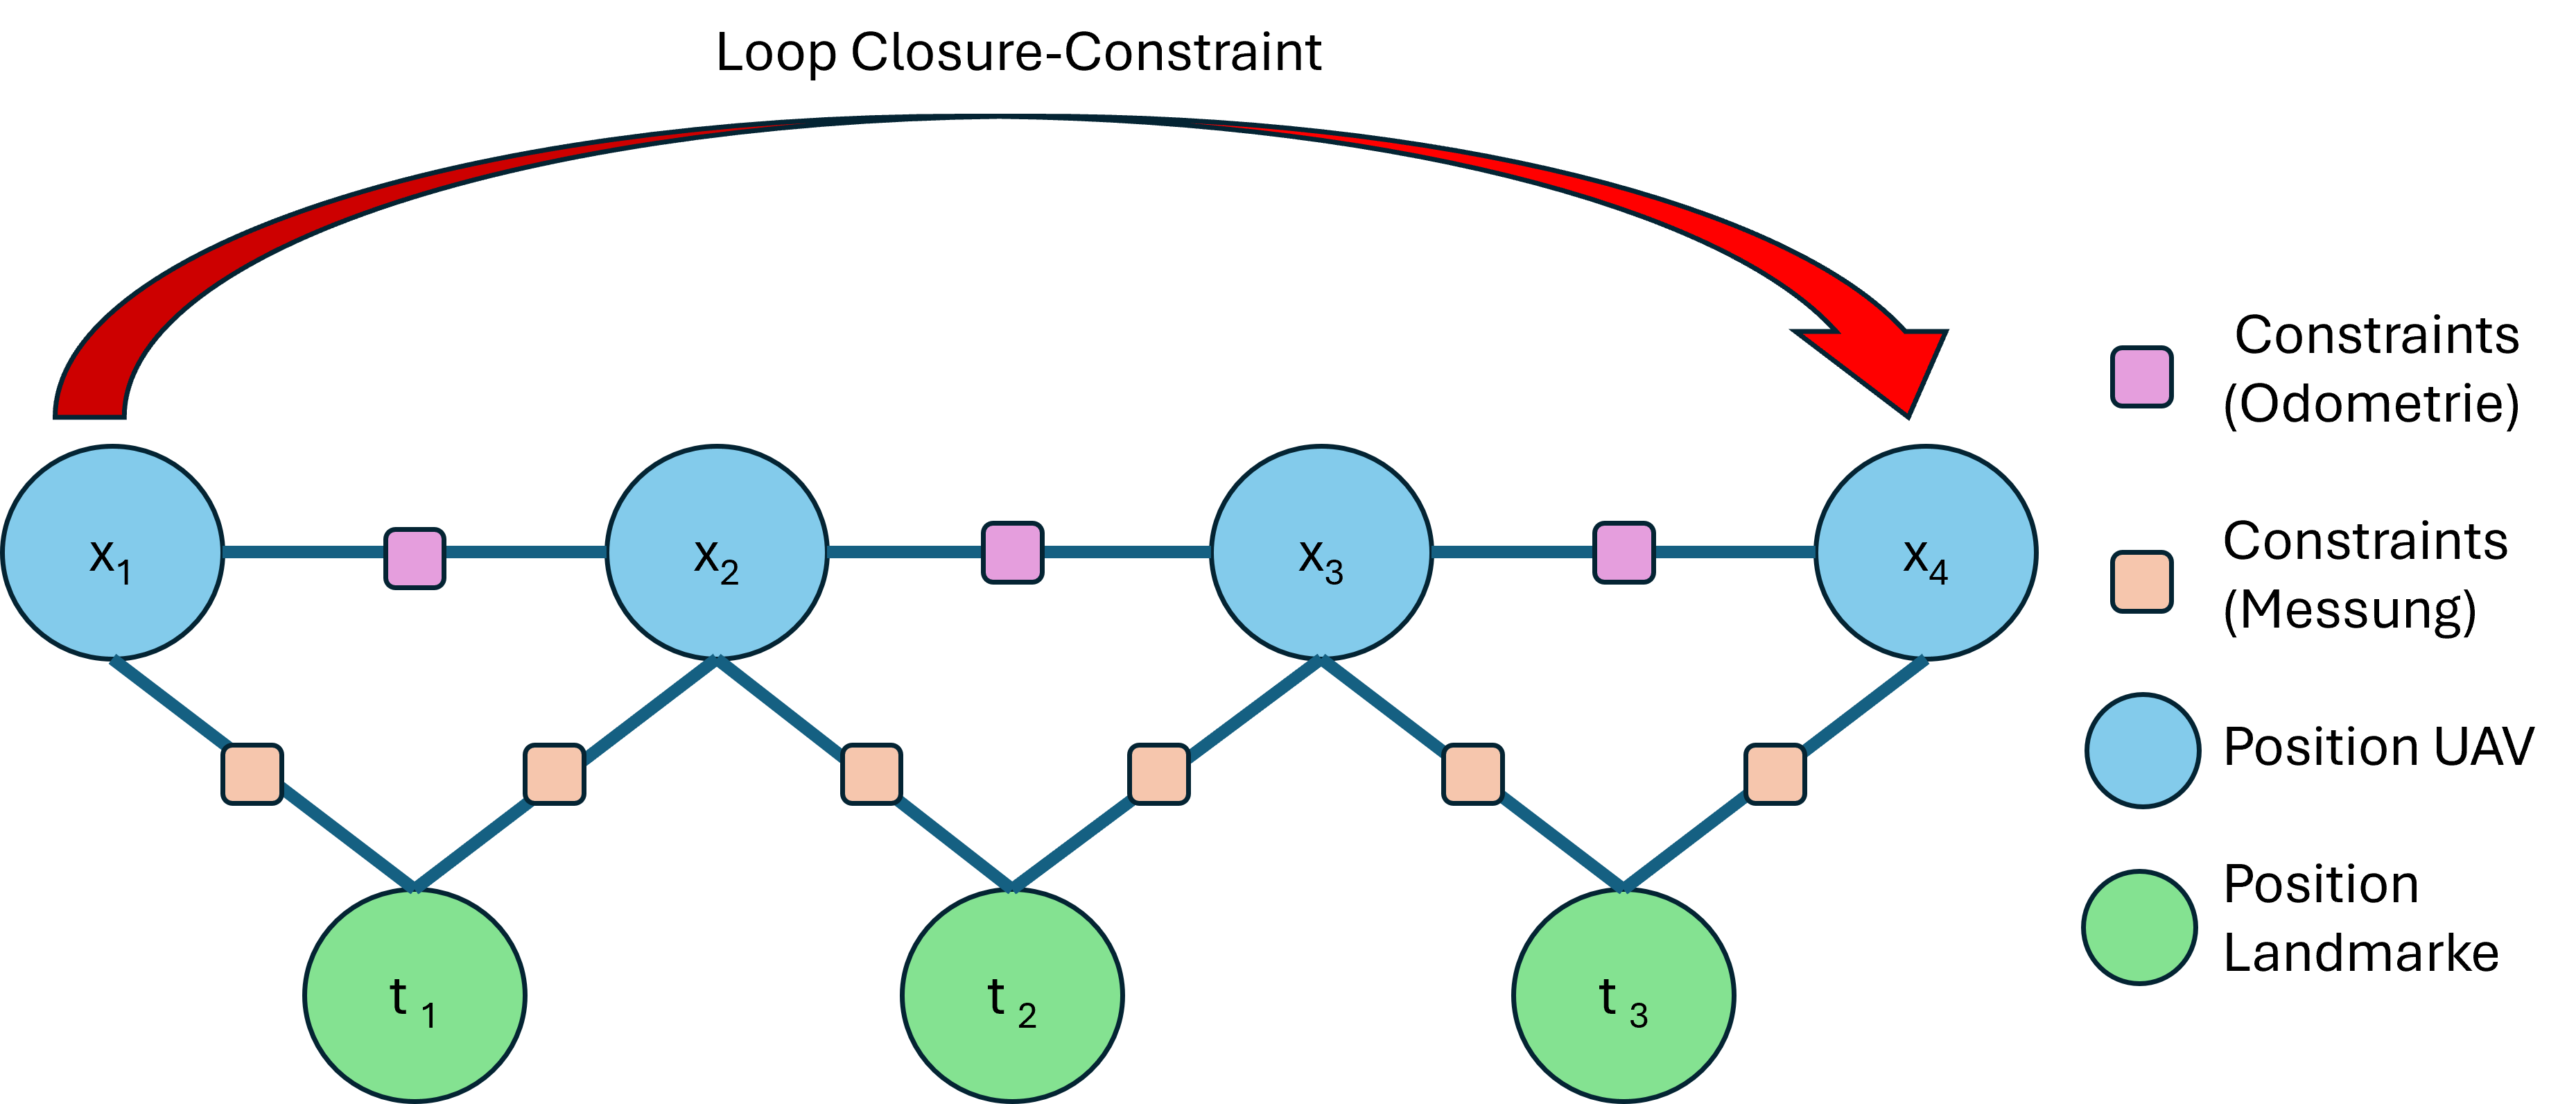
\includegraphics[width=1.0\textwidth]{Bilder/Faktorgraph_vereinfacht.png}
    \caption{Vereinfachter Faktorgraph eines \gls{slam}-Problems, 
    vgl.~\cite{Lai2022}, \cite{Dellaert2017}, \cite{Cai2024}}
    \label{fig:Faktorgraph_vereinfacht}
\end{figure}
\FloatBarrier

Das Ziel der Optimierung ist die Maximum-a-posteriori-Schätzung -- also die Konfiguration aller Variablen (Posen und Landmarken) zu finden, die die 
Gesamtwahrscheinlichkeit aller Beobachtungen maximiert. Äquivalent dazu wird der Gesamtfehler über alle Constraints minimiert.\cite{dellaert2012factor}
Bildlich bedeutet das, dass der Optimierer die Variablen solange ``verschiebt'', bis der Gesamtfehler über allen Messungen minimal ist.



\subsubsection{SLAM-Varianten}
\textbf{\gls{vslam}} nutzt visuelle Sensordaten, um gleichzeitig die Pose eines Roboters zu schätzen und eine Karte der Umgebung zu erstellen.\cite{10169695}
Es baut auf den Konzepten der \gls{vo} und \gls{vio} auf und erweitert diese um die Fähigkeit zur globalen Kartenkonsistenz durch Loop Closure.\cite{Cai2024}


\textbf{ORB-SLAM} ist ein weit verbreitetes Open-Source-\gls{vslam}-System, 
das ORB-Merkmale (Oriented FAST and Rotated BRIEF) zur Merkmalserkennung 
verwendet und sowohl Mono-, Stereo- als auch RGB-D-Kameras unterstützt.\cite{10169695}


\textbf{TagSLAM} ist eine Spezialisierung von \gls{vslam} für Fiducial-Marker.
Anstelle natürlicher Bildmerkmale werden AprilTag-Marker als definierte 
Referenzpunkte verwendet.
TagSLAM nutzt den GTSAM-Faktorgrafen-Optimierer als Backend und ermöglicht 
neben vollständigem SLAM auch extrinsische Kamerakalibrierung und 
Posenschätzung.\cite{TagSLAM}
In dieser Arbeit wird TagSLAM zur Offline-Kartierung der Versuchsumgebung 
eingesetzt.





\section{Fiducial-Marker-Systeme}


\section{Mustererkennung mit RANSAC}

